\chapter{Die Vorlage}
\label{vorlage}
  
  In diesem Kapitel wird die Vorlage näher beschrieben.
  
  \section{Das Hauptdokument}
  \label{hauptdokument}

  Das Hauptdokument ist in der Datei »documentation.tex« zu finden. Diese Datei skizziert den Aufbau des Gesamtdokuments, was bedeutet, daß dieses Dokument zum kompilieren verwandt werden muß.
    
    \subsection{Aufbau des Dokuments}
    
    Das Dokument ist bereits so aufgebaut, wie es für unsere Zwecke genügen sollte. Am Anfang binden wir eine sogenannte »Header«-Datei ein, die sämtliche Information über den Textsatz enthält. Abschnitt \ref{aufbauheader} geht genauer auf diese Datei ein.
    
    \designbox{Einbindung der »Header«-Datei}{
      \texttt{ $\backslash$input\{contents/0\_header\} }
    }
    
    Danach beginnt der Befehl für den Anfang des Dokuments. Ein TeX-Dokument muß immer mit dem Befehl \texttt{$\backslash$begin\{document\}} begonnen werden.
    
    Die Einleitung des Dokuments ist folgendermaßen aufgebaut.
    
    \begin{itemize}
      \item Titelseite
      \item Abstract
      \item Inhaltsverzeichnis
      \item Bildverzeichnis
      \item Tabellenverzeichnis
    \end{itemize}
    
    Hiernach wechseln wir die Nummerierung auf arabisch und beginnen mit dem Hauptteil der Arbeit. Jetzt werden alle Kapitel eingebunden. Da alle Kapitel in separaten Dateien abgelegt sind, müssen diese natürlich in der gewünschten Reihenfolge eingefügt werden.
    
    Direkt danach folgt der Anhang, der auf jeden Fall folgende Dinge enthält
    
    \begin{itemize}
      \item Abkürzungsverzeichnis
      \item Glossar
      \item Eidesstattliche Erklärung
      \item Literaturverzeichnis
      \item Anhang mit Material/Fragebögen usw.
    \end{itemize}
    
    
    \subsection{Stil des Literaturverzeichnisses}
    
    Als Mitglieder der TechFak verwenden wir den Zitatstil »alphadin«. Dies ist Standard für naturwissenschaftliche Texte in Deutschland und unterscheidet sich stark von »apastyle«, der bevorzugt in psychologischen Arbeiten verwendet wird.


  \section{Ein Kapitel}

  Wie eine Kapiteldatei benannt wird ist nicht sonderlich wichtig. Es ist entscheidend, daß der Dateiname ohne seine Endung korrekt in die Hauptdatei (vgl. Abschnitt \ref{hauptdokument}) eingebunden wird.

    \subsection{Aufbau}
    
    Jedes Kapitel beginnt mit dem Befehl \texttt{$\backslash$chapter\{Kapitelname\}}. Der Befehl \texttt{$\backslash$label\{kapitelname\}} definiert einen Verweisnamen, damit wir später im Dokument darauf zugreifen können. Wenn ich nun folgendes im Dokument schreibe, dann nehme ich bezug auf dieses "Label":

    \designbox{Referenz auf ein Label}{
      … wie wir in Kapitel $\backslash$ref\{kapitelname\} sehen …
    }

    TeX weiß nun, daß es die Kapitelnummer von exakt diesem Kapitel einfügen muß. D.h. die Kapitelnummer ändert sich immer auf exakt das richtige egal, ob man vorher noch 5 Kapitel einschiebt oder was auch immer.
    
    \subsection{Hierarchieebenen}

    Die Hierarchieebenen des Dokuments sind folgendermaßen:
    
    \begin{itemize}
      \item $\backslash$chapter
      \item $\backslash$section 
      \item $\backslash$subsection 
      \item $\backslash$subsubsection 
      \item $\backslash$paragraph
      \item $\backslash$subparagraph
    \end{itemize}

    Labels kann man auch jedem dieser Elemente verpassen, so daß man sich auch direkt darauf beziehen kann.   


  \section{Der Kopf bzw. Header}
  \label{aufbauheader}

  Die Datei »0\_header.tex« ist das Herzstück das Dokuments. Hier wird das komplette Aussehen des Dokuments bestimmt. D.h. man kann diese Datei austauschen und das ganze sieht komplett anders aus. Der Vorteil: es ist rein gar nichts am geschriebenen Text in den Kapiteln zu ändern!
  
  Die Datei ist gut kommentiert und eigentlich selbsterklärend. Es ist wichtig, die Einstellungen für das PDF zu ändern, so daß sichergestellt ist, daß die Stichwörter, Autoren usw. zum Dokument passen.


  \section{Literatur und Referenzen}

  In der Datei »D\_referenzen.bib« befindet sich die Literatur. Sie ist dort im BibTeX-Standard abgelegt. Ein Beispieleintrag sähe nun folgendermaßen aus:
  
  \designbox{Beispiel für BibTex}{
    \fontspec[Color=101010, Scale=0.8]{Courier}
    @book\{badura99,
    
      ~~title=\{\{Psychologie in der Praxis\}\},
      
      ~~author=\{Badura, B. and Ritter, W.\},
      
      ~~year=\{1999\},
      
      ~~publisher=\{Bohn-Verlag, Berlin\}
      
    \}
  }

  Diese Einträge kann man entweder selbst erstellen oder einfacher: man benützt dafür GoogleSchoolar oder CiteSeerX. Man sollte allerdings unvollständige Einträge selbst ergänzen, um so ein ordentliches Literaturverzeichnis, welches wissenschaftlichen Standards entspricht, zu erhalten. 
  
  Das einzige, was per Hand anpaßt wird, ist der Kurzname (im obigen Beispiel »badura99«). Dieser Kurzname wird benötigt, wenn man sich im Dokument darauf bezieht. Im Text zitiere ich nun folgendermaßen:

  \designbox{Zitate einfügen}{
  Nach $\backslash$cite\{badura99\} ergab das ganze ein tolles Ergebnis.
  }

  Im Literaturverzeichnis tauchen nur Sachen auf, die man wirklich zitiert hat (es gibt natürlich auch Möglichkeiten trotzdem Dinge aufzunehmen, die man nicht zitiert). Ebenfalls sieht man im Dokument, welche Verweise man im Literaturverzeichnis vergessen hat! Hier erscheinen hinterher Einträge à la [?] auf. Diese sollte man vor Abgabe der Arbeit dringend überprüfen und entsprechend korrigieren.


  \section{Test}
  \label{test}
  
    \subsection*{Sektion ohne Eintrag}
    
    Ich bin eine Sektion, die nicht im Inhaltsverzeichnis auftaucht. Dies erreiche ich durch einen \texttt{*}.
    
    \subsection*{Sektion, die zweite}
    
    \begin{figure}[h!]
      \centering
      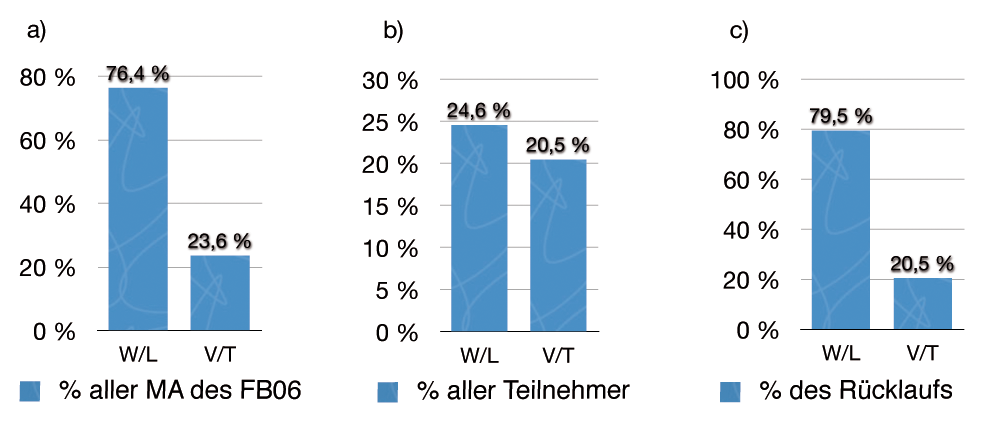
\includegraphics[width=11cm]{bilder/bild1.png} 
      \caption{Ich bin die Beschreibung und bin wichtig}
      \label{bild1}
    \end{figure}
    
    Abbildung \ref{bild1} zeigt die prozentuale Verteilung der Dienstbereiche im Fachbereich. 76,4\% der insgesamt 165 Mitarbeiter arbeiten in den Dienstbereichen Wissenschaft und Lehre (W/L, n = 126), 23,6\% in den Bereichen Verwaltung und Technik (V/T, n~=~39). 

    \subsection*{Tabellen}
    
    Wie in Tabelle \ref{tabelleBeteiligungsverhaeltnis} dargestellt ist, lag die Beteiligung der weiblichen Mitarbeiter mit knapp 53\% leicht über der der männlichen Mitarbeiter mit gut 47\%.
        
    \begin{table}[h]
      \centering
      \caption{\label{tabelleBeteiligungsverhaeltnis} Beteiligungsverhältnis Männer/Frauen}
      \begin{tabular}{|l|c|c|c|c|} \hline
        \multicolumn{2}{|c|}{} & \multicolumn{2}{c|}{\textbf{Geschlecht}} & \multirow{2}{*}{\textbf{Gesamt}} \\  \cline {3-4}
        \multicolumn{2}{|c|}{} & weiblich & männlich & \\ \hline
        \textbf{Dienst-} & Wissenschaft/Lehre & 14 & 16 & 30 \\ \cline{2-5}
        \textbf{bereich} & Verwaltung/Technik & 6 & 2 & 8 \\ \hline
        \multicolumn{2}{|l|}{Gesamt} & 20 (53\%) & 18 (47\%) & 38 (100\%) \\ \hline
     \end{tabular}
   \end{table}
   
   Alle Tabellen sind natürlich als TeX in das Dokument eingefügt und gehen damit ins Tabellenverzeichnis ein; sie werden nicht fälschlicherweise als Bild aufgeführt. Einen guten Editor für TeX sollte man allerdings dafür besitzen. Ein für alle Betriebssysteme verfügbarer Editor ist z.B. Kile. Eine andere Möglichkeit sind spezielle Tabellenkonverter. Dazu befragt man am besten das Repository seines Betriebsystems.

    
    \subsection*{Ein anderes Bild}
    
    Mit etwa 34\% ist die Gruppe der 30- bis 39jährigen Mitarbeiter in dieser Stichprobe am größten. Darauf folgen die 20- bis 29jährigen Mitarbeiter mit gut 26\% (s. Abb. \ref{bild2}; n~=~38).
    
    \begin{figure}[ht]
      \centering
      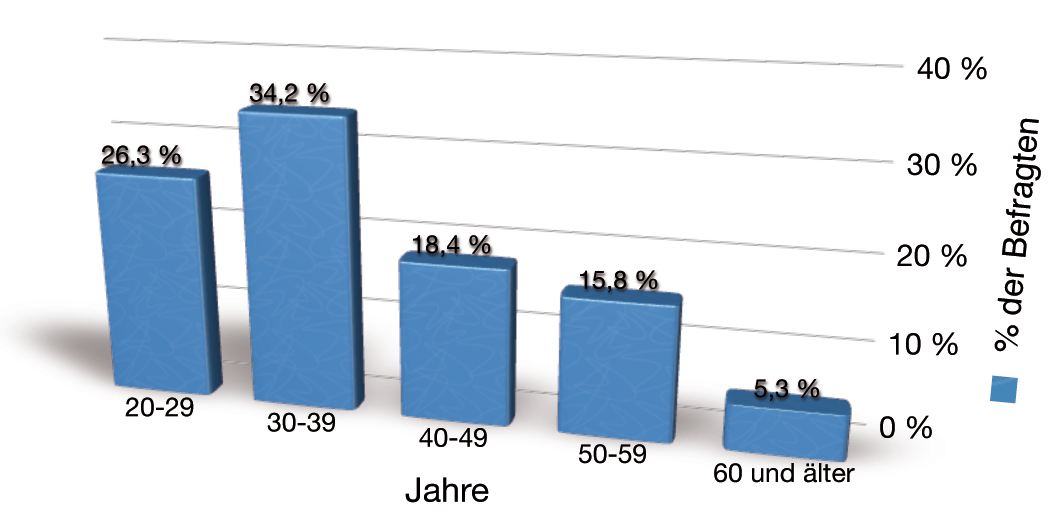
\includegraphics[width=9cm]{bilder/bild2.png} 
      \caption{Erklärung findet man hier}
      \label{bild2}
    \end{figure}
    
    \subsubsection*{Tätigkeitsdauer}
    
    Mehr als 50\% der Befragten sind seit einem Zeitraum von bis zu fünf Jahren an der Universität beschäftigt. Die nächstgrößere Gruppe arbeitet seit sechs bis zehn Jahren an der Universität (s. Abb. \ref{bild3}; n~=~39). 
    
    \begin{figure}[h]
      \centering
      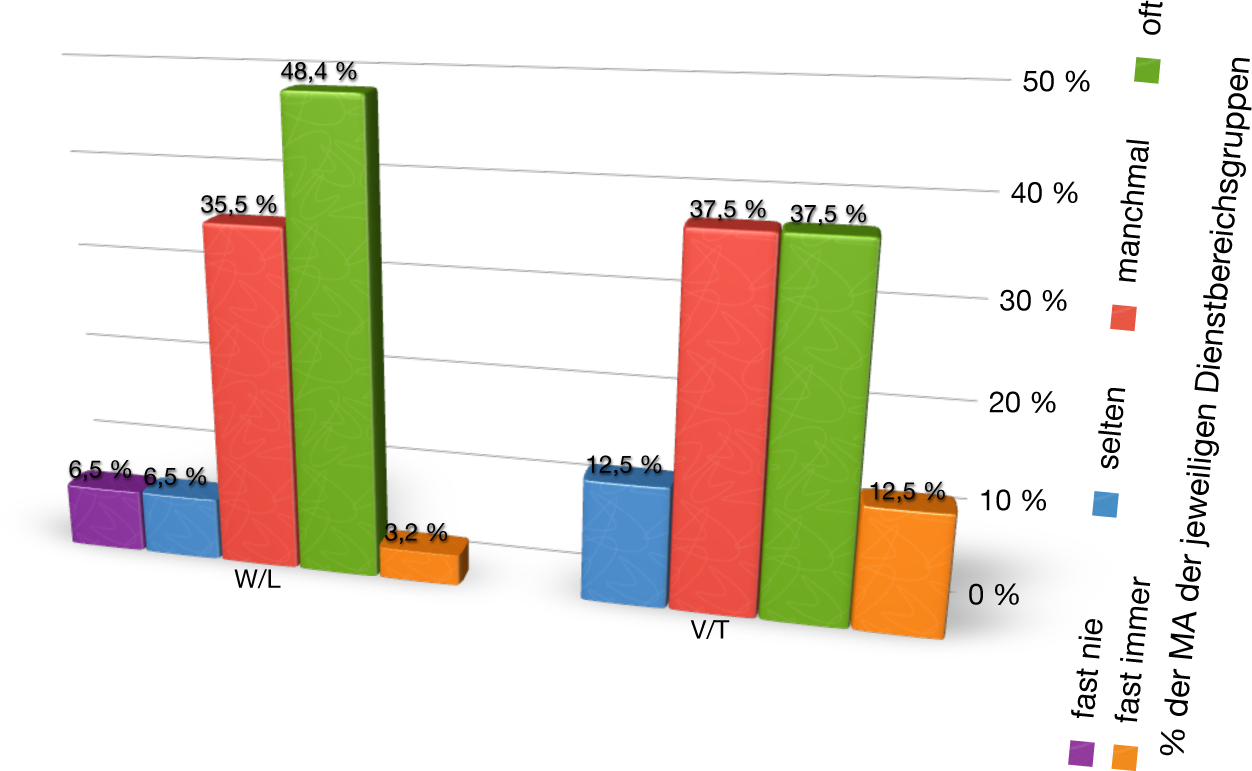
\includegraphics[width=12cm]{bilder/bild3.png} 
      \caption{Beschreibung}
      \label{bild3}
    \end{figure}

  \section{Schlußwort}
  \label{schluszwort}
  
  Die Darstellung der Graphiken und Tabellen im gesamten Abschnitt \ref{test} beziehen sich auf alle 429 Teilnehmer der Umfrage.
